\chapter{LabVIEW User Manual} \label{labviewManaul}

This appendix goes through the main LabVIEW program, and explains how it should be used from a user's perspective. The program is launched by opening project found under \texttt{labview/red\_bike.lvproj} in LabVIEW 2019. Later versions might work as well, but the 2019 version is recommended for the best compatibility. Inside the project, open \texttt{myRIO-1900/bin/TestMain.vi}. The first time the program is opened on a new computer, LabVIEW might give a warning that a \texttt{.lvbitx} file could not be found. This file is located in \texttt{labviw/bin}, and can manually be pointed to when requested.

With the program opened, the controls which can be interacted with to control be bike are located in the top left of the front panel. These controls are shown in image \ref{fig:labviewControls} below.

\begin{figure}[H]
    \centering
    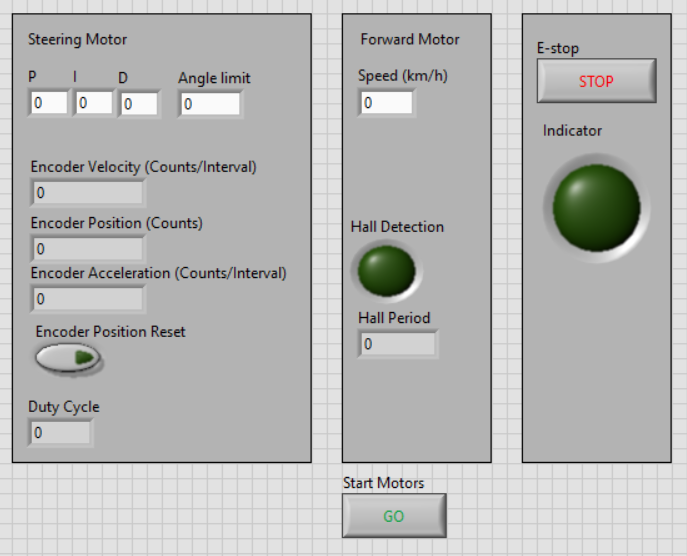
\includegraphics[width=10cm]{figure/labview_controls.png}
    \caption{The controls which can be interacted with in the LabVIEW front panel.}
    \label{fig:labviewControls}
\end{figure}

In the leftmost box in the picture contains the controls for the steering motor. Here, the PID gains and the angle limit (in degrees from the center), can be changed. Below this are the readouts from the encoder, and a button to reset its position. This button should be pressed when the front wheel is straight to calibrate the encoder before starting any of the motors. At the bottom of the box is the duty cycle which is sent from the balancing algorithm to the steering motor.

The middle box at the center of the image contains the controls for the forward motor. The only thing which can be changed here is the RPM, note that the RPM are measured in relation with the pedals (for the red bike). Below the forward motor controls is a button which starts the two motors. It should be mentioned that the program can still be running without affecting the motors, if this button is not pressed.

At the right is a software implementation of the emergency stop. From the program's perspective, this acts exactly as if the hardware emergency stop was to be pressed.

The path to the log file (including its desired name) can be specified in the text field which is located at the absolute bottom of the image. The path leads to a file \textbf{on the MyRIO} where the LabVIEW program is running, and must be inside the \texttt{/home/lvuser/} directory. This is due to the program not having \textit{sudo} privileges in the Linux OS which is running on the device. If no file exists in the specified path, a file will be created. If a file does exist, it will be replaced and overwritten when the program starts. It is therefore recommended to change the file name before each time the program is to be run. To open the log files, they have to be downloaded from the MyRIO using for example FileZilla, and then opened using any of the methods mentioned in \ref{method:logging}.

The rest of the front panel consists of the values from the various sensors. On the right of the controls depicted in the figure above are three graphs illustrating the values from the IMU's gyroscope. The topmost graph corresponds with the roll rate which is used by the balancing algorithm. The front panel also shows GPS data and accelerometer values, these are however not used by any part of the program at the moment.

In summary, the following steps must be performed to start the bike and log its sensor and control signal data:
\begin{enumerate}
    \item Set the PID gains, and angle limit and RPM to something non-zero
    %\item Set the angle limit to something non-zero
    %\item Set the RPM
    \item Set the path to the logging file to somewhere inside the \texttt{/home/lvuser/} directory. For example \texttt{/home/lvuser/log1.tdms}
    \item Start the LabVIEW program
    \item Reset the encoder position when steering wheel is straight
    \item Press \textit{GO}
\end{enumerate}

Note that, to be able to start the LabVIEW program, the hardware emergency stop has to be up, and the hardware reset button has to be pressed. The program is ready when the light next to the reset button shines green.